% Options for packages loaded elsewhere
% Options for packages loaded elsewhere
\PassOptionsToPackage{unicode}{hyperref}
\PassOptionsToPackage{hyphens}{url}
\PassOptionsToPackage{dvipsnames,svgnames,x11names}{xcolor}
%
\documentclass[
  11pt,
  letterpaper,
  DIV=11,
  numbers=noendperiod]{scrartcl}
\usepackage{xcolor}
\usepackage{amsmath,amssymb}
\setcounter{secnumdepth}{5}
\usepackage{iftex}
\ifPDFTeX
  \usepackage[T1]{fontenc}
  \usepackage[utf8]{inputenc}
  \usepackage{textcomp} % provide euro and other symbols
\else % if luatex or xetex
  \usepackage{unicode-math} % this also loads fontspec
  \defaultfontfeatures{Scale=MatchLowercase}
  \defaultfontfeatures[\rmfamily]{Ligatures=TeX,Scale=1}
\fi
\usepackage{lmodern}
\ifPDFTeX\else
  % xetex/luatex font selection
\fi
% Use upquote if available, for straight quotes in verbatim environments
\IfFileExists{upquote.sty}{\usepackage{upquote}}{}
\IfFileExists{microtype.sty}{% use microtype if available
  \usepackage[]{microtype}
  \UseMicrotypeSet[protrusion]{basicmath} % disable protrusion for tt fonts
}{}
% Make \paragraph and \subparagraph free-standing
\makeatletter
\ifx\paragraph\undefined\else
  \let\oldparagraph\paragraph
  \renewcommand{\paragraph}{
    \@ifstar
      \xxxParagraphStar
      \xxxParagraphNoStar
  }
  \newcommand{\xxxParagraphStar}[1]{\oldparagraph*{#1}\mbox{}}
  \newcommand{\xxxParagraphNoStar}[1]{\oldparagraph{#1}\mbox{}}
\fi
\ifx\subparagraph\undefined\else
  \let\oldsubparagraph\subparagraph
  \renewcommand{\subparagraph}{
    \@ifstar
      \xxxSubParagraphStar
      \xxxSubParagraphNoStar
  }
  \newcommand{\xxxSubParagraphStar}[1]{\oldsubparagraph*{#1}\mbox{}}
  \newcommand{\xxxSubParagraphNoStar}[1]{\oldsubparagraph{#1}\mbox{}}
\fi
\makeatother


\usepackage{longtable,booktabs,array}
\usepackage{calc} % for calculating minipage widths
% Correct order of tables after \paragraph or \subparagraph
\usepackage{etoolbox}
\makeatletter
\patchcmd\longtable{\par}{\if@noskipsec\mbox{}\fi\par}{}{}
\makeatother
% Allow footnotes in longtable head/foot
\IfFileExists{footnotehyper.sty}{\usepackage{footnotehyper}}{\usepackage{footnote}}
\makesavenoteenv{longtable}
\usepackage{graphicx}
\makeatletter
\newsavebox\pandoc@box
\newcommand*\pandocbounded[1]{% scales image to fit in text height/width
  \sbox\pandoc@box{#1}%
  \Gscale@div\@tempa{\textheight}{\dimexpr\ht\pandoc@box+\dp\pandoc@box\relax}%
  \Gscale@div\@tempb{\linewidth}{\wd\pandoc@box}%
  \ifdim\@tempb\p@<\@tempa\p@\let\@tempa\@tempb\fi% select the smaller of both
  \ifdim\@tempa\p@<\p@\scalebox{\@tempa}{\usebox\pandoc@box}%
  \else\usebox{\pandoc@box}%
  \fi%
}
% Set default figure placement to htbp
\def\fps@figure{htbp}
\makeatother


% definitions for citeproc citations
\NewDocumentCommand\citeproctext{}{}
\NewDocumentCommand\citeproc{mm}{%
  \begingroup\def\citeproctext{#2}\cite{#1}\endgroup}
\makeatletter
 % allow citations to break across lines
 \let\@cite@ofmt\@firstofone
 % avoid brackets around text for \cite:
 \def\@biblabel#1{}
 \def\@cite#1#2{{#1\if@tempswa , #2\fi}}
\makeatother
\newlength{\cslhangindent}
\setlength{\cslhangindent}{1.5em}
\newlength{\csllabelwidth}
\setlength{\csllabelwidth}{3em}
\newenvironment{CSLReferences}[2] % #1 hanging-indent, #2 entry-spacing
 {\begin{list}{}{%
  \setlength{\itemindent}{0pt}
  \setlength{\leftmargin}{0pt}
  \setlength{\parsep}{0pt}
  % turn on hanging indent if param 1 is 1
  \ifodd #1
   \setlength{\leftmargin}{\cslhangindent}
   \setlength{\itemindent}{-1\cslhangindent}
  \fi
  % set entry spacing
  \setlength{\itemsep}{#2\baselineskip}}}
 {\end{list}}
\usepackage{calc}
\newcommand{\CSLBlock}[1]{\hfill\break\parbox[t]{\linewidth}{\strut\ignorespaces#1\strut}}
\newcommand{\CSLLeftMargin}[1]{\parbox[t]{\csllabelwidth}{\strut#1\strut}}
\newcommand{\CSLRightInline}[1]{\parbox[t]{\linewidth - \csllabelwidth}{\strut#1\strut}}
\newcommand{\CSLIndent}[1]{\hspace{\cslhangindent}#1}



\setlength{\emergencystretch}{3em} % prevent overfull lines

\providecommand{\tightlist}{%
  \setlength{\itemsep}{0pt}\setlength{\parskip}{0pt}}



 


\usepackage{caption}
\captionsetup{font=small, labelfont=bf}
\setlength{\parindent}{0pt}
\setlength{\parskip}{1.25ex}
\KOMAoption{captions}{tableheading}
\makeatletter
\@ifpackageloaded{caption}{}{\usepackage{caption}}
\AtBeginDocument{%
\ifdefined\contentsname
  \renewcommand*\contentsname{Table of contents}
\else
  \newcommand\contentsname{Table of contents}
\fi
\ifdefined\listfigurename
  \renewcommand*\listfigurename{List of Figures}
\else
  \newcommand\listfigurename{List of Figures}
\fi
\ifdefined\listtablename
  \renewcommand*\listtablename{List of Tables}
\else
  \newcommand\listtablename{List of Tables}
\fi
\ifdefined\figurename
  \renewcommand*\figurename{Figure}
\else
  \newcommand\figurename{Figure}
\fi
\ifdefined\tablename
  \renewcommand*\tablename{Table}
\else
  \newcommand\tablename{Table}
\fi
}
\@ifpackageloaded{float}{}{\usepackage{float}}
\floatstyle{ruled}
\@ifundefined{c@chapter}{\newfloat{codelisting}{h}{lop}}{\newfloat{codelisting}{h}{lop}[chapter]}
\floatname{codelisting}{Listing}
\newcommand*\listoflistings{\listof{codelisting}{List of Listings}}
\makeatother
\makeatletter
\makeatother
\makeatletter
\@ifpackageloaded{caption}{}{\usepackage{caption}}
\@ifpackageloaded{subcaption}{}{\usepackage{subcaption}}
\makeatother
\usepackage{bookmark}
\IfFileExists{xurl.sty}{\usepackage{xurl}}{} % add URL line breaks if available
\urlstyle{same}
\hypersetup{
  pdftitle={Image statistic encoding between regions of the visual cortex},
  pdfauthor={Al Xin},
  colorlinks=true,
  linkcolor={blue},
  filecolor={Maroon},
  citecolor={Blue},
  urlcolor={Blue},
  pdfcreator={LaTeX via pandoc}}


\title{Image statistic encoding between regions of the visual cortex}
\author{\small Al Xin}
\date{Sep 1, 2026}
\begin{document}
\maketitle

\renewcommand*\contentsname{Table of contents}
{
\hypersetup{linkcolor=}
\setcounter{tocdepth}{3}
\tableofcontents
}

\pagebreak

Advisors: Rob Kass (Statistics), Jenelle Feather (Psychology,
Neuroscience Institute).

\section{Abstract}\label{abstract}

Later stages of the visual cortex are thought to contain neurons
selective for progressively higher-level visual features. One
experimental approach to detecting regional differences in visual
processing is through presenting visual texture stimuli (e.g., sand,
tree bark, granite, etc.). Families of visual textures can be
parameterized by \(N\)th order joint pixel densities, so the
decodability of texture families in neural responses can indicate
selectivity for image statistics. Previously, Ziemba et al.~(2016) found
better within-family separation of neural responses in V1 and better
between-family separation in V2
{[}\citeproc{ref-ziemba_selectivity_2016}{1}{]}, and related work found
that texture stimuli with matched higher order image statistics produced
higher firing in V2 and V4
{[}\citeproc{ref-freeman_functional_2013}{2}--\citeproc{ref-lee_emergence_2025}{4}{]}.
However, existing analyses lack comparisons with IT, which responds more
sparsely to stimuli. Neural responses in IT are sparse in two different
ways: first, most IT neurons will not respond to any texture stimuli;
and second, of the IT neurons with any response to texture, only a small
number of unique stimuli will produce a response. The between-family
separability in IT compared to V4 can change depending on the handling
of reliable and responsive sites, suggesting that IT efficiently encodes
higher-level image statistics.

\section{Extended abstract}\label{extended-abstract}

\subsection{Higher- and lower-order visual areas may be characterized by
differences in processing image
statistics}\label{higher--and-lower-order-visual-areas-may-be-characterized-by-differences-in-processing-image-statistics}

Later stages of the visual cortex are thought to contain neurons
selective for progressively higher-level visual features. The primary
visual cortex (V1), for instance, contains neurons that selectively
respond to simple image features like oriented edges. In contrast, the
inferior temporal gyrus (IT), which handles later visual processing,
contains areas selective for object categories, such as the fusiform
face area for facial recognition. One approach to characterize the
relevant visual features for each layer is through recording neural
responses to visual texture stimuli, which are approximately homogeneous
images with repeated elements, e.g., images of sand, tree bark, granite,
or honeycomb. Texture categories (families) can be parameterized by a
set of image statistics, where image statistics are \(N\)th-order
empirical densities of pixels. Unique texture samples within the same
family share image statistics and should elicit comparable responses in
the visual area sensitive to those particular statistics. Patterns in
selectivity for higher- and lower-order image statistics can provide
evidence for how visual information is propagated or summarized in
visual areas.

\subsection{Existing results find a tradeoff between selectivity for
higher- and lower-order
statistics}\label{existing-results-find-a-tradeoff-between-selectivity-for-higher--and-lower-order-statistics}

Previously, Ziemba et al.~(2016) found better within-family separation
of neural responses in V1 and better between-family separation in V2
{[}\citeproc{ref-ziemba_selectivity_2016}{1}{]}. Relatedly, Okazawa et
al.~(2015, 2017) compared the selectivity of V2 and V4 neurons for image
statistics in texture stimuli and found V4 neurons tended to be
selective for higher order statistics
{[}\citeproc{ref-okazawa_image_2015}{5},\citeproc{ref-okazawa_gradual_2017}{6}{]}.
Other analyses of between-region texture responses found that texture
stimuli with matched higher order image statistics produced higher
firing of V2 and V4 neurons compared to stimuli lacking higher order
image statistics
{[}\citeproc{ref-freeman_functional_2013}{2}--\citeproc{ref-lee_emergence_2025}{4}{]}.

\subsection{It is unknown whether trends in selectivity for image
statistics extend beyond
V4}\label{it-is-unknown-whether-trends-in-selectivity-for-image-statistics-extend-beyond-v4}

\begin{figure}

\centering{

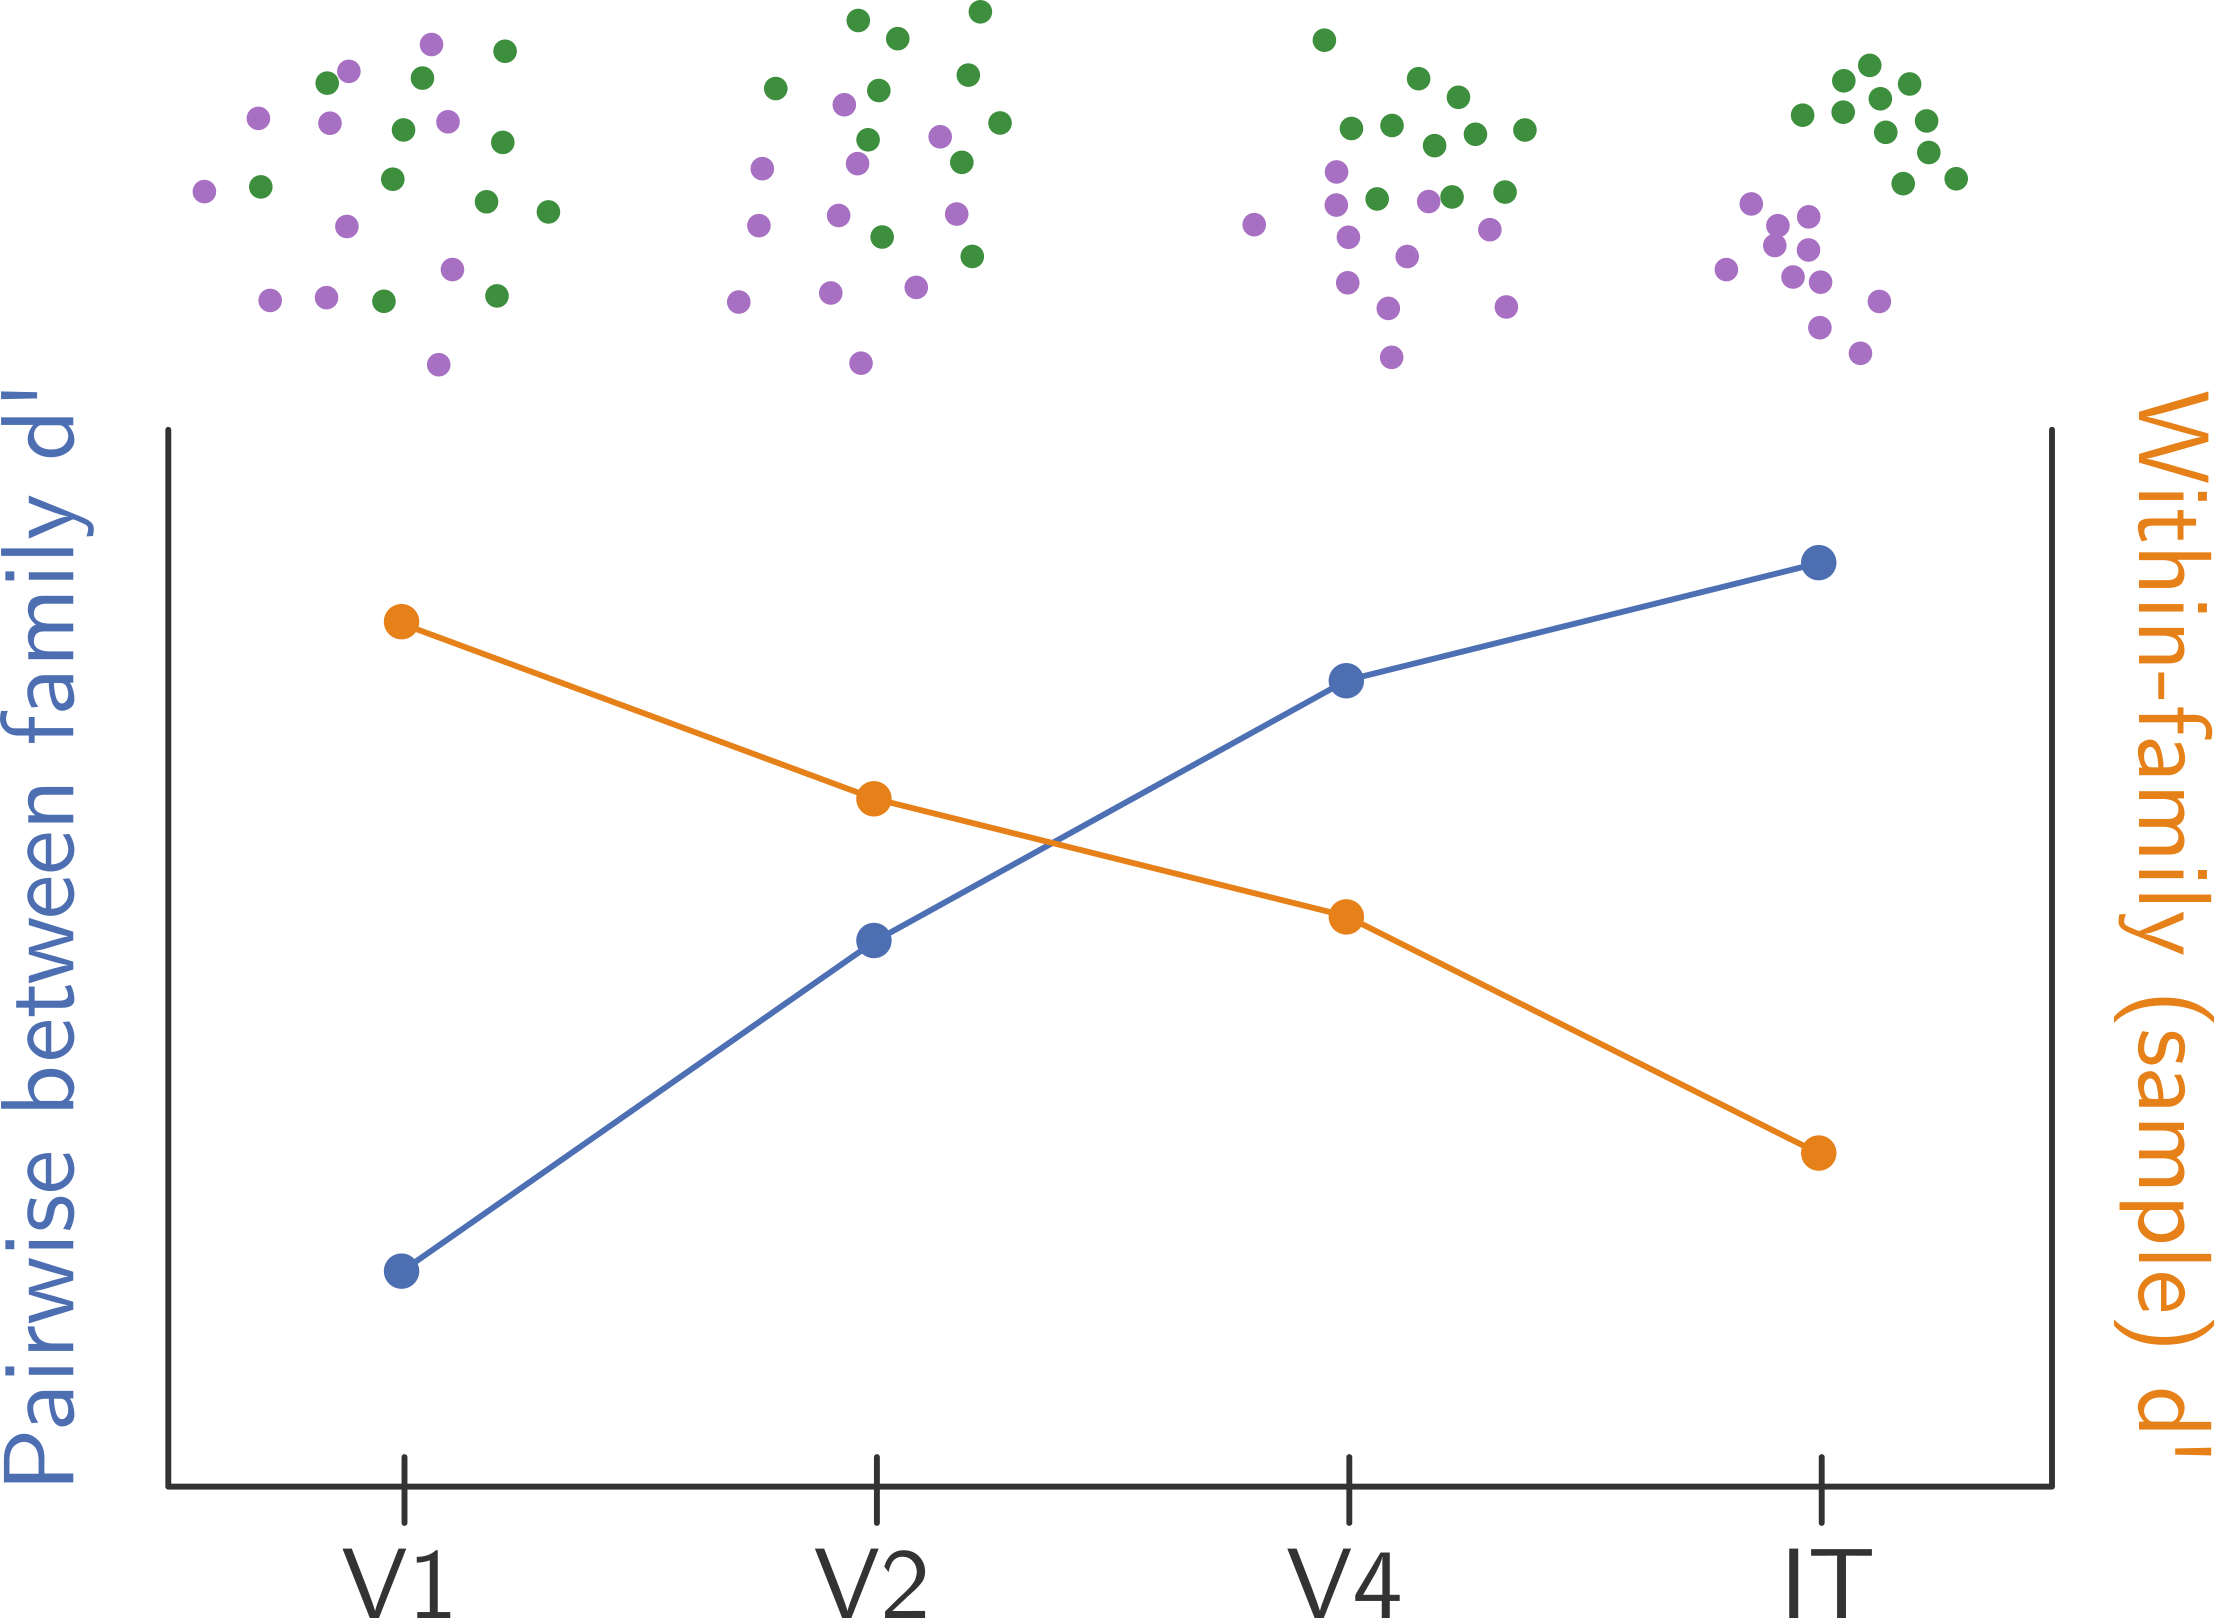
\includegraphics[width=0.5\linewidth,height=\textheight,keepaspectratio]{../img/proposed_results.png}

}

\caption{\label{fig-intro}(Top) A visual representation of two families
in some arbitrary 2D representation space. (Bottom) The distances
between families and between samples, with some arbitrary values for
each region.}

\end{figure}%

In my ADA, I am analyzing data collected by Lee et al.~(2024), who
recorded neural responses in V1, V2, V4, and IT, spanning the entire
range of the visual processing stream
{[}\citeproc{ref-lee_developmentally_2024}{3}{]}. Based on previous
results, I expect to find better between-group discrimination in later
areas and better within-group discrimination in earlier areas (see
Figure~\ref{fig-intro} for a schematic). However, existing analyses tend
to lack results for the entire visual processing stream, so it is
unclear if this trend will reliably extend to IT. This gap is partially
due to the practical limitations of supporting a large population of
animals, but there are also methodological challenges with analyzing IT.
Higher level areas tend to produce sparse responses, so typical
approaches in the literature, such as size-matched population analyses
or single-site neuron metrics, may not produce reliable comparisons
between IT and earlier visual areas.

\subsection{Results for IT are dependent on the treatment of
sparsity}\label{results-for-it-are-dependent-on-the-treatment-of-sparsity}

I found that neural responses in IT are sparse in two different ways:
first, most IT neurons will not respond to any texture stimuli; and
second, of the IT neurons with any response to texture, only a small
number of unique stimuli will produce a response. For V1, V2, and V4,
recording sites that are unreliable (low correlation between responses
to the same stimuli) tend to also be unresponsive (low separability
between responses to different stimuli). However, IT contains a higher
proportion of sites that are reliable but unresponsive. Retaining
reliable sites in IT produces worse between-family separability in IT
compared to V4, while limiting analyses to responsive sites reverses
this trend, producing better between-family separability in IT compared
to V4. The within-family separability in IT remains consistently worse
than V4. This contrast suggests that IT destructively summarizes
pixel-level differences in images but efficiently encodes higher-level
image statistics.

\pagebreak

\section{Methods and analysis}\label{methods-and-analysis}

\subsection{Mahalanobis distance can capture linear separability but is
not robust to variation in dimensionality
(100\%)}\label{mahalanobis-distance-can-capture-linear-separability-but-is-not-robust-to-variation-in-dimensionality-100}

\subsection{Generalization performance of regularized regression models
can be applied to between-family but not within-family comparisons
(100\%)}\label{generalization-performance-of-regularized-regression-models-can-be-applied-to-between-family-but-not-within-family-comparisons-100}

\subsection{Typical criteria for discarding unreliable or unresponsive
sites may produce selection bias
(100\%)}\label{typical-criteria-for-discarding-unreliable-or-unresponsive-sites-may-produce-selection-bias-100}

\subsection{Randomized dichotomy distances can compensate for low sample
numbers in within-family comparisons
(80\%)}\label{randomized-dichotomy-distances-can-compensate-for-low-sample-numbers-in-within-family-comparisons-80}

\subsection{Shrinkage covariance estimators can also be applied to
within-family comparisons
(100\%)}\label{shrinkage-covariance-estimators-can-also-be-applied-to-within-family-comparisons-100}

\pagebreak

\section{Results}\label{results}

\subsection{Subject-specific patterns in sparsity appear across V1, V4,
and IT
(100\%)}\label{subject-specific-patterns-in-sparsity-appear-across-v1-v4-and-it-100}

\subsection{IT responses are sparse at both the site- and image-level
(95\%)}\label{it-responses-are-sparse-at-both-the-site--and-image-level-95}

\subsection{The best-separated texture families and sample images tend
to be consistent across regions and subjects
(80\%)}\label{the-best-separated-texture-families-and-sample-images-tend-to-be-consistent-across-regions-and-subjects-80}

\subsection{V2 produces the highest between-sample separability and V4
produces the highest between-family separability
(90\%)}\label{v2-produces-the-highest-between-sample-separability-and-v4-produces-the-highest-between-family-separability-90}

\subsection{Different metrics for separability produce similar relative
results
(60\%)}\label{different-metrics-for-separability-produce-similar-relative-results-60}

\subsection{Site inclusion criteria affect separability comparisons
between V4 and IT
(40\%)}\label{site-inclusion-criteria-affect-separability-comparisons-between-v4-and-it-40}

\section{Discussion}\label{discussion}

\subsection{Texture families are a limited proxy of the target measure
of image statistic
selectivity}\label{texture-families-are-a-limited-proxy-of-the-target-measure-of-image-statistic-selectivity}

\subsection{Multi-unit activations may record from neighboring
neurons}\label{multi-unit-activations-may-record-from-neighboring-neurons}

\subsection{Sparsity in IT may drive differences between neural decoding
results and behavioral
performance}\label{sparsity-in-it-may-drive-differences-between-neural-decoding-results-and-behavioral-performance}

\subsection{Between-region and between-subject sparsity considerations
precludes selection of a holdout
set}\label{between-region-and-between-subject-sparsity-considerations-precludes-selection-of-a-holdout-set}

\pagebreak

\section{References}\label{references}

\phantomsection\label{refs}
\begin{CSLReferences}{0}{1}
\bibitem[\citeproctext]{ref-ziemba_selectivity_2016}
\CSLLeftMargin{1. }%
\CSLRightInline{Corey M. Ziemba, Jeremy Freeman, J. Anthony Movshon,
Eero P. Simoncelli. Selectivity and tolerance for visual texture in
macaque V2. Proc Natl Acad Sci USA. 2016 May 31;113(22).
doi:\href{https://doi.org/10.1073/pnas.1510847113}{10.1073/pnas.1510847113}}

\bibitem[\citeproctext]{ref-freeman_functional_2013}
\CSLLeftMargin{2. }%
\CSLRightInline{Jeremy Freeman, Corey M. Ziemba, David J. Heeger, Eero
P. Simoncelli, J. Anthony Movshon. A functional and perceptual signature
of the second visual area in primates. Nat Neurosci. 2013
Jul;16(7):974--81.
doi:\href{https://doi.org/10.1038/nn.3402}{10.1038/nn.3402}}

\bibitem[\citeproctext]{ref-lee_developmentally_2024}
\CSLLeftMargin{3. }%
\CSLRightInline{Gerick M. Lee, C. L. Rodríguez Deliz, Brittany N.
Bushnell, Najib J. Majaj, J. Anthony Movshon, Lynne Kiorpes.
Developmentally stable representations of naturalistic image structure
in macaque visual cortex. Cell Reports. 2024 Aug 27;43(8).
doi:\href{https://doi.org/10.1016/j.celrep.2024.114534}{10.1016/j.celrep.2024.114534}}

\bibitem[\citeproctext]{ref-lee_emergence_2025}
\CSLLeftMargin{4. }%
\CSLRightInline{Gerick M. Lee, Najib J. Majaj, C. L. Rodríguez Deliz,
Lynne Kiorpes, J. Anthony Movshon. Emergence of a contrast-invariant
representation of naturalistic texture in macaque visual cortex.
Proceedings of the National Academy of Sciences. 2025 Dec
2;122(48):e2501437122.
doi:\href{https://doi.org/10.1073/pnas.2501437122}{10.1073/pnas.2501437122}}

\bibitem[\citeproctext]{ref-okazawa_image_2015}
\CSLLeftMargin{5. }%
\CSLRightInline{Gouki Okazawa, Satohiro Tajima, Hidehiko Komatsu. Image
statistics underlying natural texture selectivity of neurons in macaque
V4. Proceedings of the National Academy of Sciences. 2015 Jan
27;112(4):E351--60.
doi:\href{https://doi.org/10.1073/pnas.1415146112}{10.1073/pnas.1415146112}}

\bibitem[\citeproctext]{ref-okazawa_gradual_2017}
\CSLLeftMargin{6. }%
\CSLRightInline{Gouki Okazawa, Satohiro Tajima, Hidehiko Komatsu.
Gradual development of visual texture-selective properties between
macaque areas V2 and V4. Cereb Cortex. 2017 Oct 1;27(10):4867--80.
doi:\href{https://doi.org/10.1093/cercor/bhw282}{10.1093/cercor/bhw282}}

\end{CSLReferences}




\end{document}
